\documentclass[12pt]{article}
\usepackage[utf8]{inputenc}

%%% I added a few packages. This next one allows you to set the margins.
\usepackage[top=.5in,bottom=1in,right=.75in,left=.75in]{geometry}
\usepackage{multicol}
%\usepackage{newspaper}
\setlength{\columnsep}{1cm}
\usepackage{blindtext}
\usepackage{varwidth}

%%% This one does boxes in a really nice way.
\usepackage{tcolorbox}
\usepackage{mdframed}
\usepackage{minibox}
\usepackage{graphicx}
\graphicspath{ {./images/} }
\usepackage{epstopdf}
  \epstopdfDeclareGraphicsRule{.pdf}{png}{.png}{convert #1 \OutputFile}
  \DeclareGraphicsExtensions{.png,.pdf}
\usepackage{hyperref}
\hypersetup{
    colorlinks=true,
    linkcolor=blue,
    filecolor=magenta,      
    urlcolor=cyan,
    pdftitle={MSCSMess},
    pdfpagemode=FullScreen,
    }
\urlstyle{same}
 \usepackage{fix-cm}
 \usepackage{soul}
 \usepackage{graphicx}
 \usepackage{multicol}


\newcommand{\ds}{\displaystyle}
\newcommand{\ZZ}{\mathbb{Z}}
\newcommand{\QQ}{\mathbb{Q}}
\newcommand{\RR}{\mathbb{R}}
\newcommand{\CC}{\mathbb{C}}
\newcommand{\FF}{\mathbb{F}}
\newcommand{\xx}{\mathbf{x}}
\newcommand{\uu}{\mathbf{u}}
\newcommand{\vv}{\mathbf{v}}

\newcommand{\bolder}{\textbf}
 
 
\title{\fontsize{60}{70}\selectfont {\bf {MSCS} 
\includegraphics[scale=.3]{images/OleLion.png} {Mess}}}
\author{Department of Mathematics, Statistics, and Computer Science \\ St.\@ Olaf College, Northfield, MN 55057 \vspace{-2ex}} 
\date{\today\, $|$ Volume 54, No.\@ 17 \line(1,0){500}}


\begin{document}

\maketitle \vspace{-0.5cm}
\begin{center}
Happy March and happy Friday! We hope everyone had a great week and enjoyed some of the warmer weather. Check out some of the cool events coming up and have an awesome weekend!
\end{center}

 \begin{multicols}{2}

 \begin{tcolorbox}[colback=white, colframe=black]
    \begin{center}
    \title{{\large \bolder{MSCS Colloqium 3/9}}}
    \end{center}
\end{tcolorbox}

Join us for a talk on Monday, March 9, 2026 at 3:30 PM in RNS 210 featuring Taylor Okonek, Assistant Professor of Statistics at Macalester College. In “Mortality Estimation in Data-Sparse Settings,” Professor Okonek will discuss how statisticians estimate life expectancy and mortality rates in countries without complete vital registration systems. When working with limited survey data and small geographic areas, researchers face major data challenges. This talk will introduce a statistical framework for addressing these issues, highlighting survey statistics, small area estimation, and survival analysis.

 \begin{tcolorbox}[colback=white, colframe=black]
    \begin{center}
    \title{{\large \bolder{PI DAY!}}}
    \end{center}
\end{tcolorbox}
Please join us to celebrate Pi Day (a day early) on Friday, March 13th! We will have an abundance of pies and zen pi-themed activities. Come ready to enjoy a delicious treat and unwind with your fellow pi lovers. The 6th floor lounge filled up quickly last year and the pies went fast, so come early to grab a slice! Hosted by the Math Club and the MSCS Department. 

 \begin{tcolorbox}[colback=white, colframe=black]
    \begin{center}
    \title{{\large \bolder{Pi Mu Epsilon (PME)}}}
    \end{center}
\end{tcolorbox}
St. Olaf is home to the Minnesota Kappa chapter of Pi Mu Epsilon (PME), which is a national honor society dedicated to recognizing and promoting scholarly activity in mathematics. To find out more about PME, click \href{https://pme-math.org/what-is-pme}{here}.

If you are interested in joining this math honor society, please fill out this form (\href{https://docs.google.com/forms/d/e/1FAIpQLSfXZQxdboX2mFuk5T39eG9ELSichO3ZOU6O35mqC4eaRahDWw/viewform}{link}). If you are already a member of PME and would like to purchase PME merchandise through the St. Olaf math department, please complete the same form. The form deadline is Wednesday, March 18, 2026, at 5pm. Mandatory induction for new members will be held from 3:00-4:00pm on Wednesday, April 22, 2026.

All PME members will be recognized at the St.~Olaf Honors Day celebration, and graduation cords will be to senior members as a gift from the MSCS Department. For more information, contact Rachael Norton (norton10@stolaf.edu).


 \begin{tcolorbox}[colback=white, colframe=black]
    \begin{center}
    \title{{\large \bolder{Series on AI Literacy in Education}}}
    \end{center}
\end{tcolorbox}
Generative AI technology continues to make headlines and capture attention. As part of an independent study project this spring, this discussion series provides a platform for faculty and students to share ideas, ask questions, and explore the role of generative AI tools in the classroom. There will be three sessions during the first half of the semester. More information, including dates and session times, can be found on the poster below and at this \href{https://fortressokorie.github.io/ai_literacy/} {website}! The next session will take place on Thursday, March 19th, in RNS 356 from 11:30 AM to 12:30 PM. For any questions, please contact Fortress Okorie at okorie1@stolaf.edu.

\begin{tcolorbox}[colback=white, colframe=black]
    \begin{center}
    \title{{\large \bolder{Summer Offering - Math 226: Multivariable Calculus}}}
    \end{center}
\end{tcolorbox}
Looking for something productive and fun to do for the first part of the summer?  Come take an awesome math course!  Professor Salois will be offering a section of Math 226 for Summer Session I, which will meet 10:00-11:30 AM Tuesdays-Fridays.  Registration on SIS opens on Monday March 2.  If you have any questions, please contact Professor Salois (salois1@stolaf.edu).  

\begin{tcolorbox}[colback=white, colframe=black]
    \begin{center}
    \title{{\large \bolder{Summer Opportunity in Math Education}}}
    \end{center}
\end{tcolorbox}

\href {https://bsmeducation.com} {Budapest Semesters in Mathematics Education (BSME)} is a 6-week summer program in Budapest, Hungary, designed for those interested in the learning and teaching of mathematics. Participants take a variety of courses in mathematics education and complete a week-long field experience. Come experience the \href{https://bsmeducation.com/wp-content/uploads/2020/02/hungarian-pedagogy-flyer.pdf}{Hungarian pedagogy} based on guided discovery—which emphasizes problem solving, mathematical creativity, and communication—as well as the rich and vibrant culture of Hungary.

Scholarships are available from the St. Olaf Financial Aid Office. See the \href{https://wp.stolaf.edu/smithcenter/st-olaf-summer-programs/#:~:text=All%20students%20are%20automatically%20considered%20for%20a%20need%2Dbased%20scholarship%20(see%20J%2DTerm%20column)%20of%20up%20to%2050%25%20of%20program%20costs%20from%20the%20St.%20Olaf%20Financial%20Aid%20Office.%C2%A0%C2%A0}{Smith Center's} webpage for more details. If you have any questions, contact Prof. Ryota Matsuura (matsuura@stolaf.edu).

\begin{tcolorbox}[colback=white, colframe=black]
    \begin{center}
    \title{{\large \bolder{Problem Solving Group}}}
    \end{center}
\end{tcolorbox}
The Math Problem Solving Group meets weekly to have fun, solve math problems, eat candy, and prepare for upcoming math contests. Meetings are Thursdays from 11:30 am - 12:30 pm, in RNS 207 (the Center for Interdisciplinary Research room). Everyone is welcome, regardless of prior experience in mathematics or math contests!


\end{multicols} \vfill 

\begin{center}
    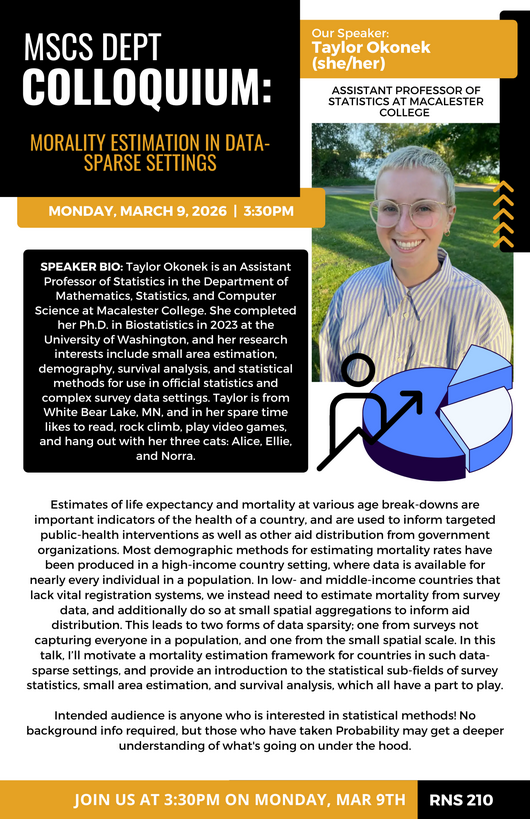
\includegraphics[height=0.95\textheight]{images/Colloq Taylor Okonek.png}
\end{center}


\begin{center}
    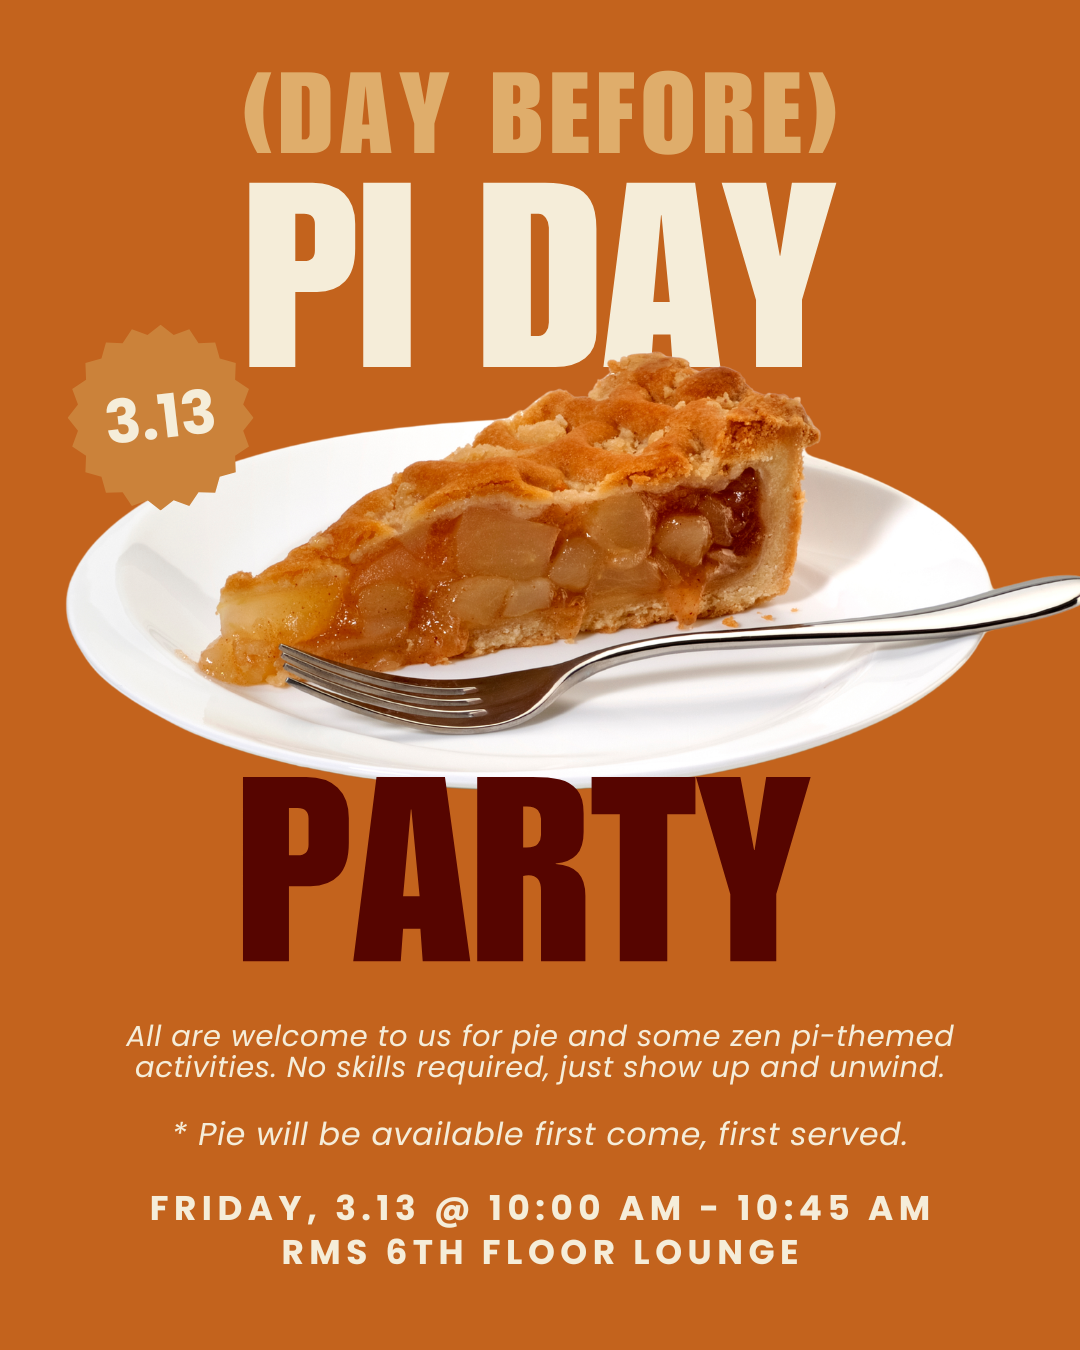
\includegraphics[height=0.95\textheight]{images/Pi Day 2026.png}
\end{center}


\begin{center}
    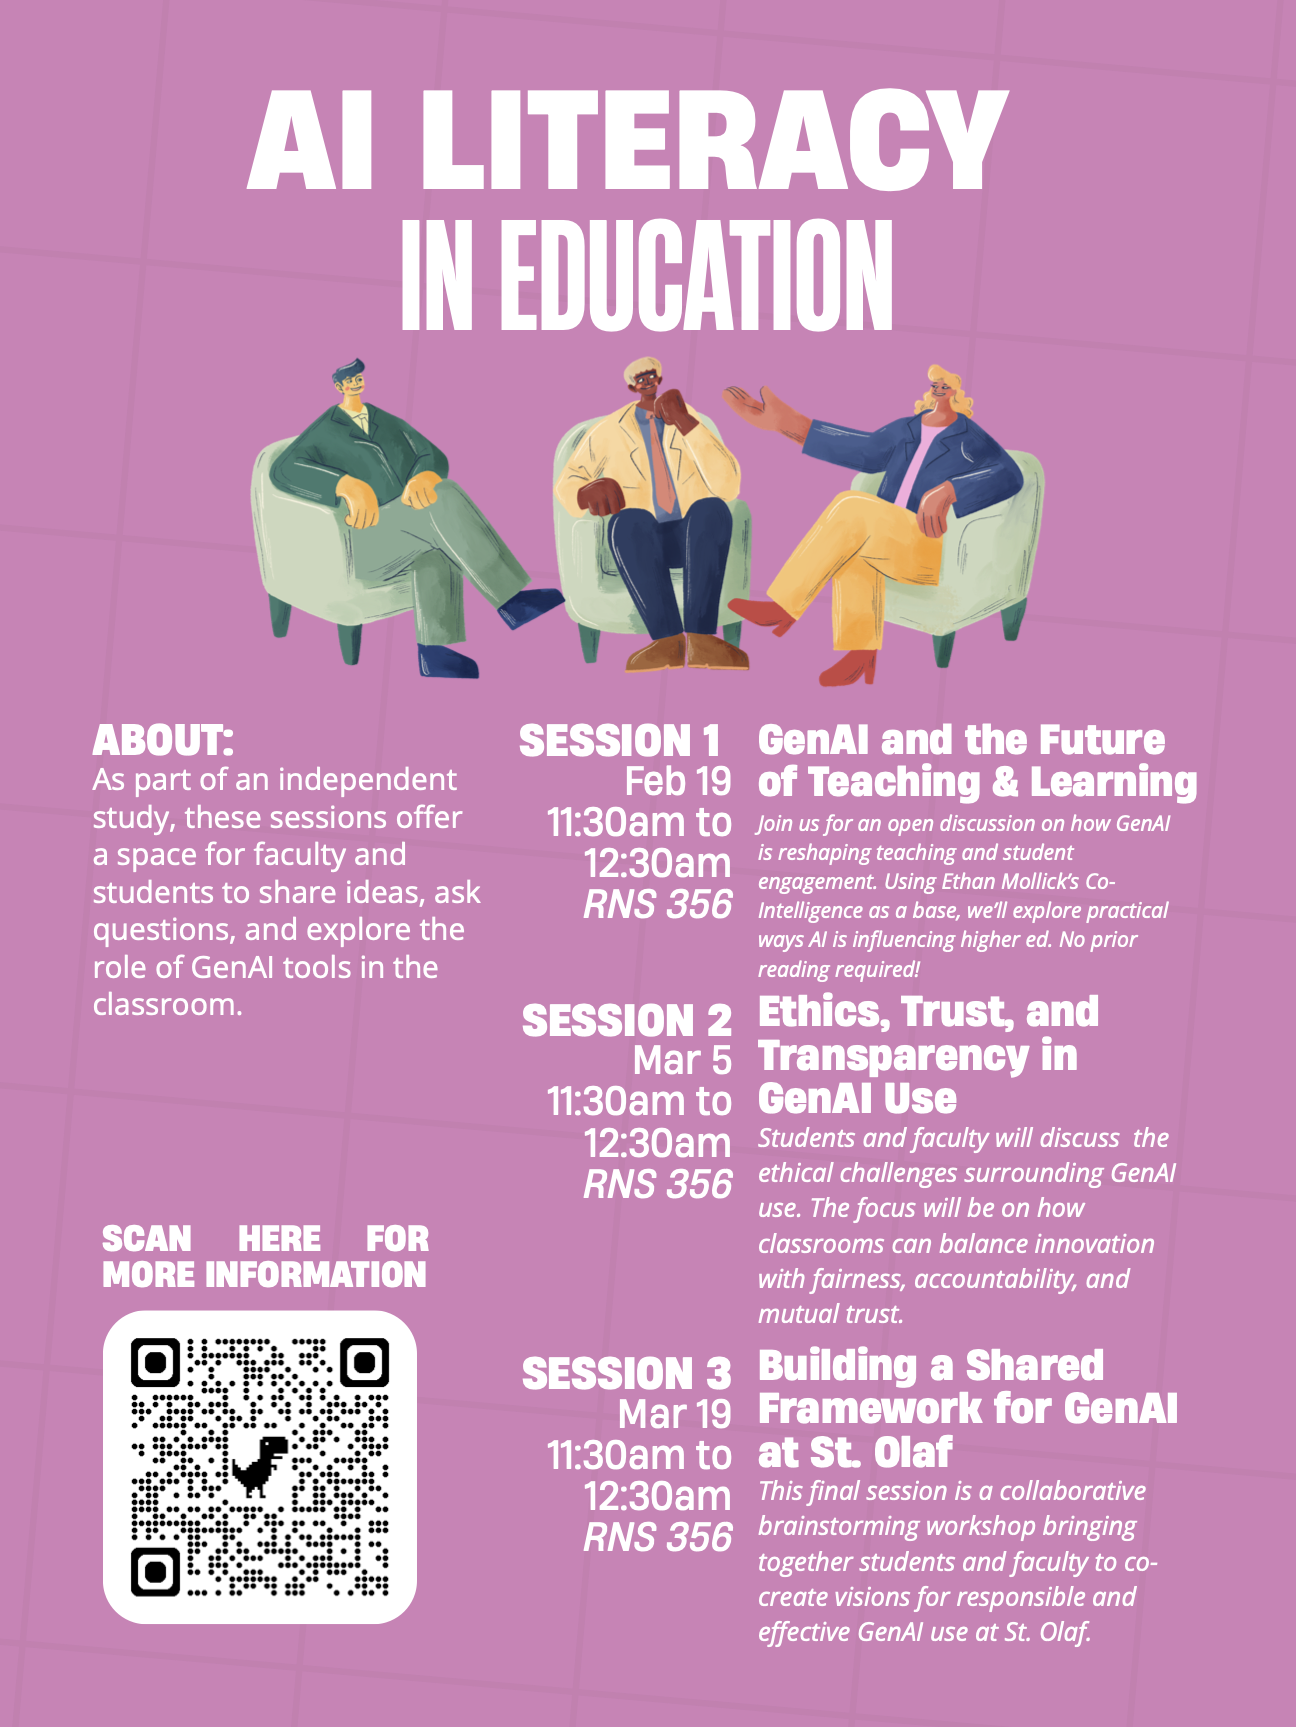
\includegraphics[height=0.95\textheight]{images/AI Literacy in Education2.png}
\end{center}


\begin{center}
    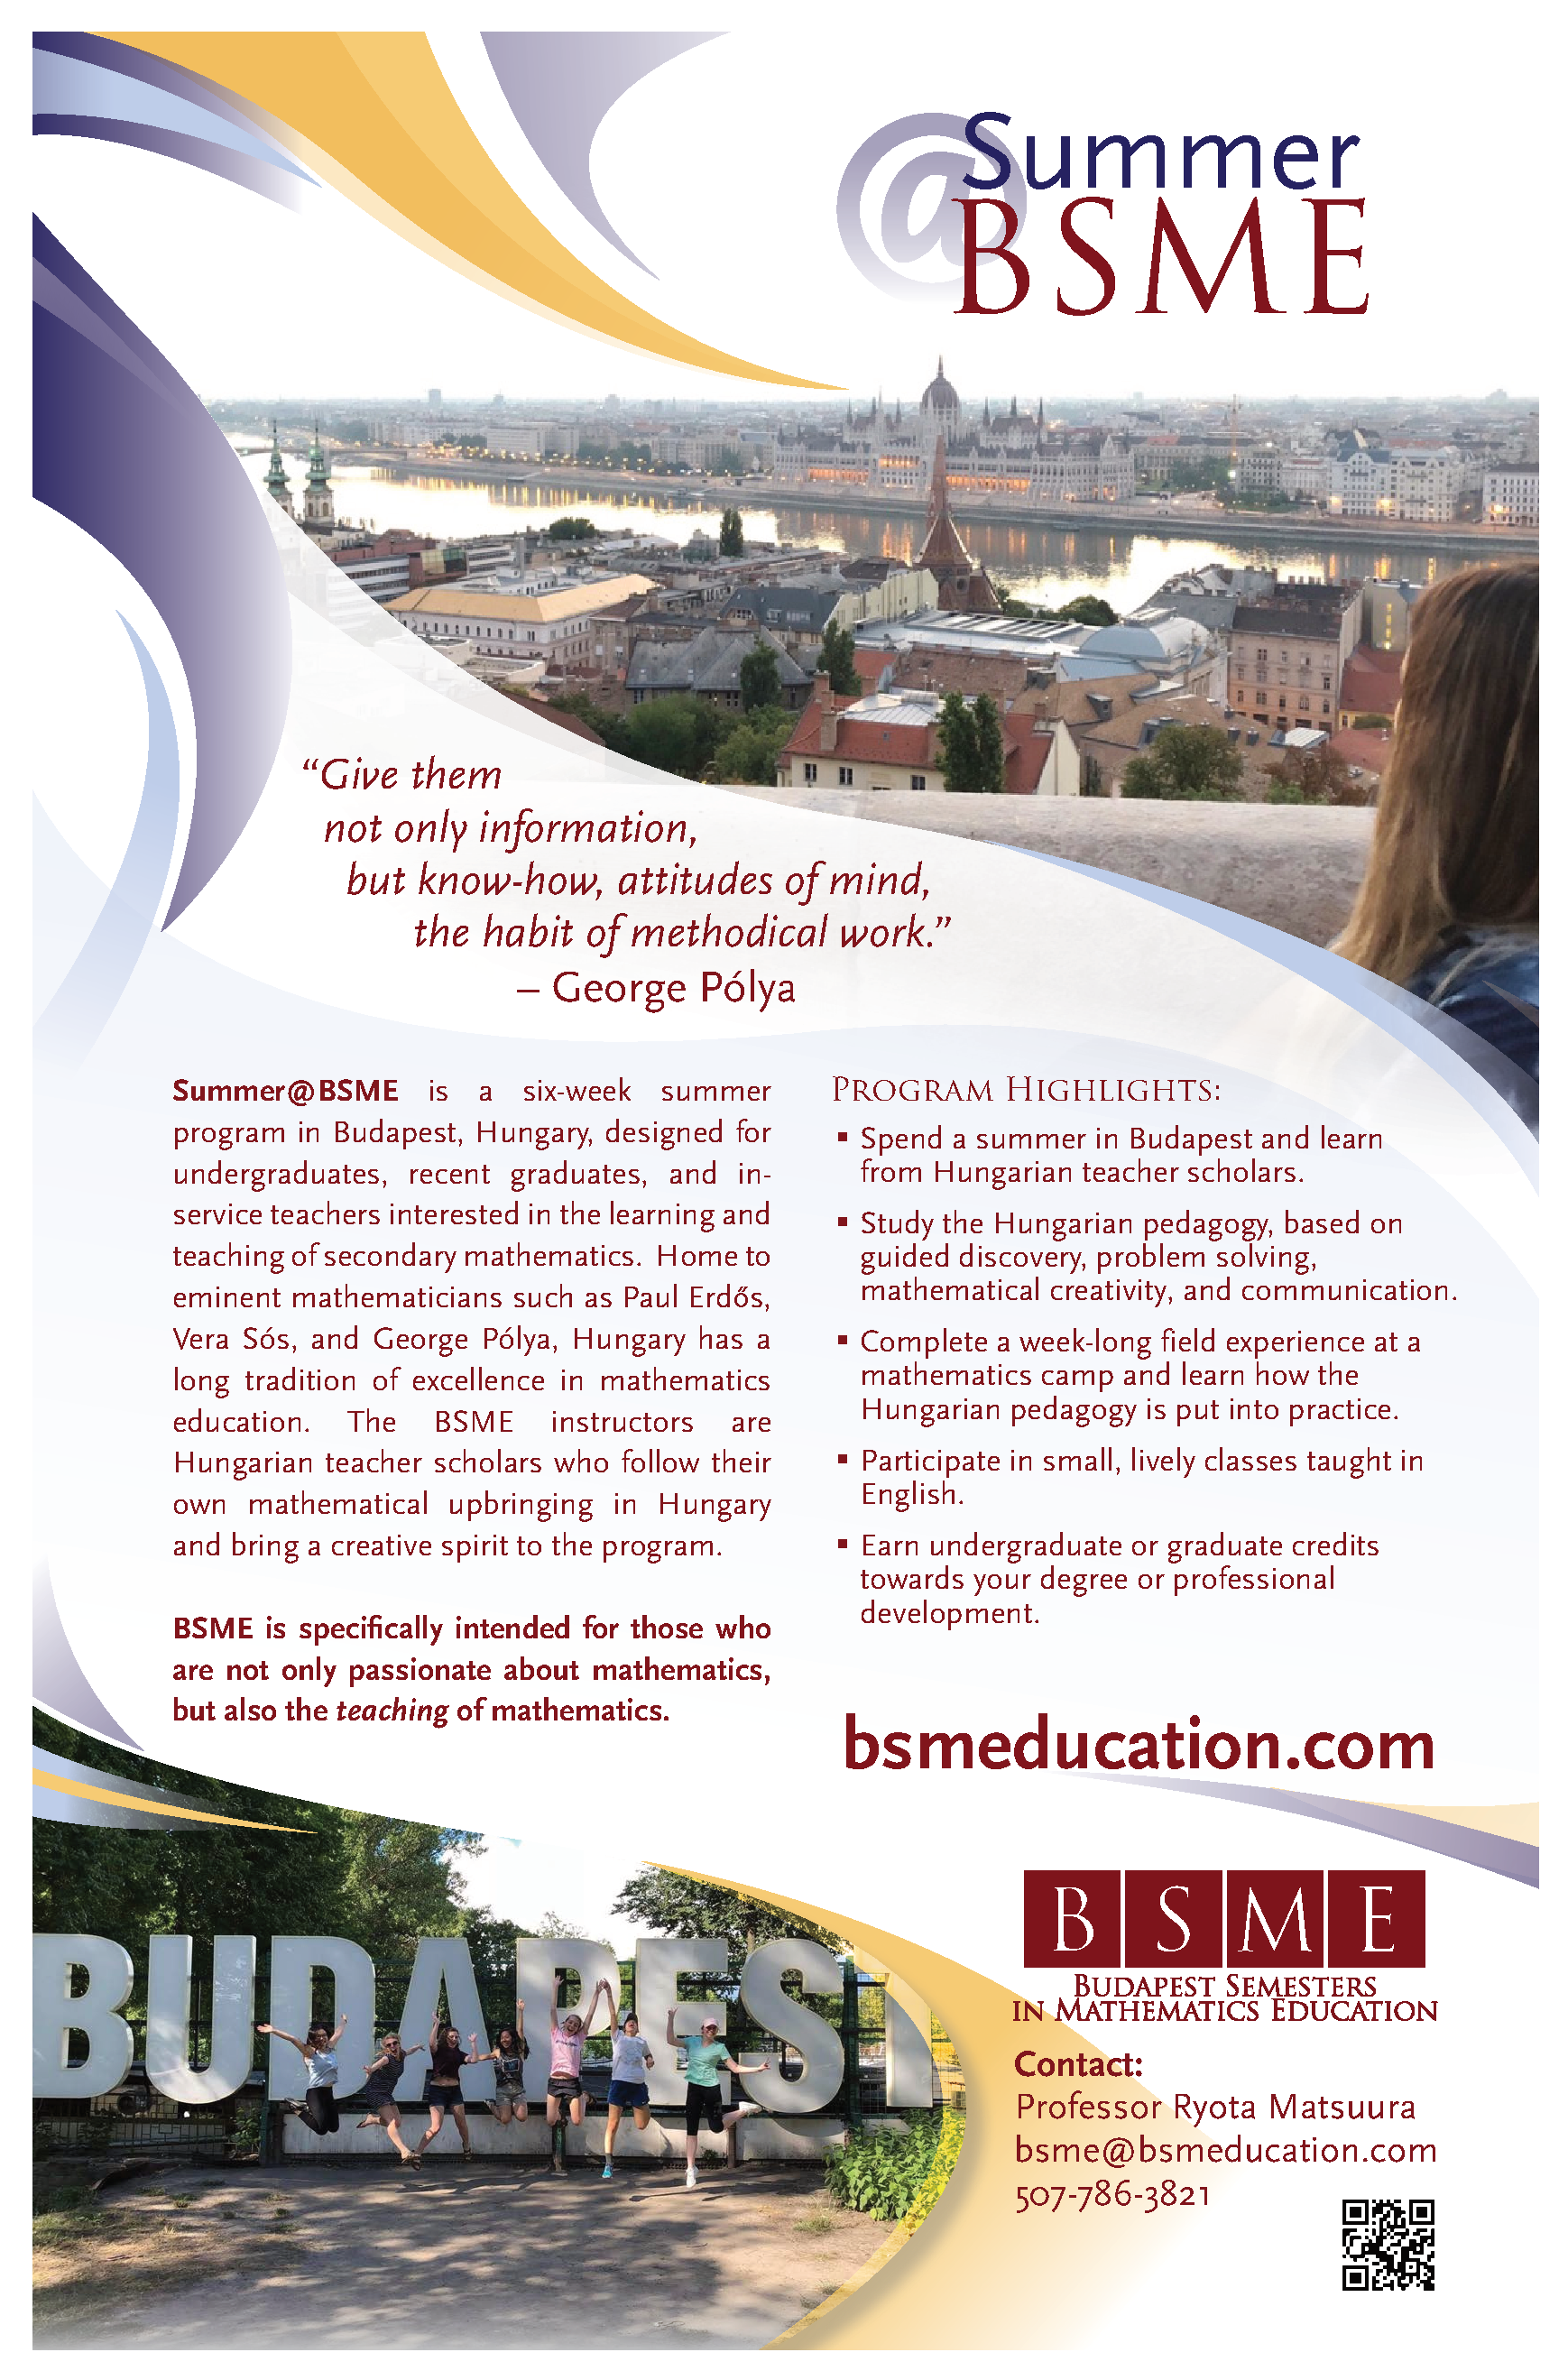
\includegraphics[height=0.95\textheight]{images/2024-bsme-poster-revised-web.pdf}
\end{center}

\begin{center}

\includegraphics[width=0.9\textwidth]{images/Tea Time Poster.png}
\end{center}

\noindent{To submit an article, event, or anything else for publication in the Mess, email messeditor@stolaf.edu. Visit \href{https://wp.stolaf.edu/mscs/mscs-mess/}{http://wp.stolaf.edu/mscs/mscs-mess/} for a digital archive of previous MSCS Mess issues.}\\
	
\hfill Nima Dahir, Editor
	
\hfill Kyle Salois, Faculty Advisor


 

\end{document}